\documentclass[10pt,letterpaper,onecolumn]{article}

\usepackage[T1]{fontenc}
\usepackage[utf8]{inputenc}
\usepackage[letterpaper,hmargin=1in,vmargin=1in]{geometry}
\usepackage{array}
\usepackage{booktabs}
\usepackage{longtable}
\usepackage{float}
\usepackage{tikz}
\usepackage{microtype}
\usepackage{amsmath}
\usepackage{amssymb}
\usepackage{listings}
\usepackage{xcolor}
\usepackage{enumitem}
\usepackage[compact]{titlesec}
\usepackage[hidelinks]{hyperref}
\usepackage[nohyphen]{underscore}
\usepackage{natbib}

\titlespacing*{\section}{0pt}{1.05ex plus .2ex}{0.45ex plus .1ex}
\titlespacing*{\subsection}{0pt}{0.85ex plus .2ex}{0.3ex plus .1ex}
\setlist[enumerate]{topsep=2pt,itemsep=1pt,parsep=0pt,leftmargin=*}
\setlength{\textfloatsep}{8pt plus 2pt minus 2pt}
\setlength{\floatsep}{8pt plus 2pt minus 2pt}
\setlength{\intextsep}{8pt plus 2pt minus 2pt}
\setlength{\abovedisplayskip}{5pt}
\setlength{\belowdisplayskip}{5pt}
\renewcommand{\topfraction}{0.92}
\renewcommand{\bottomfraction}{0.7}
\renewcommand{\textfraction}{0.06}
\renewcommand{\floatpagefraction}{0.85}
\setcounter{topnumber}{3}
\setcounter{bottomnumber}{2}
\setcounter{totalnumber}{4}

\usetikzlibrary{arrows.meta,positioning,fit,backgrounds}

% Every number in this paper is defined in one of these files. The three
% benchmark files are written by the runs that produced them and are inputs by
% relative path, never copies. derived-macros.tex is regenerated by
% tools/derive-macros.py from the artifact each count is read from.
\newcommand{\PSHostCpuModel}{Neoverse-N1}
\newcommand{\PSHostCores}{12}
\newcommand{\PSHostMemoryGiB}{46.9}
\newcommand{\PSHostOs}{Linux 6.17.0-1020-oracle aarch64}
\newcommand{\PSRustcVersion}{1.94.1}
\newcommand{\PSHostLoadAverage}{4.69}
\newcommand{\PSPathSampleCount}{100}
\newcommand{\PSCriterionSampleCount}{100}
\newcommand{\PSWarmupCount}{2}
\newcommand{\PSBuyerWorkflowPFiftyMs}{2096.522}
\newcommand{\PSBuyerWorkflowPNinetyNineMs}{2146.402}
\newcommand{\PSBuyerWorkflowMeanMs}{2096.823}
\newcommand{\PSBuyerWorkflowStdMs}{32.471}
\newcommand{\PSBuyerWorkflowCiLowMs}{2090.914}
\newcommand{\PSBuyerWorkflowCiHighMs}{2103.544}
\newcommand{\PSBuyerWorkflowPFiftySec}{2.097}
\newcommand{\PSBuyerWorkflowPNinetyNineSec}{2.146}
\newcommand{\PSProducerPFiftyMs}{1835.866}
\newcommand{\PSProducerPNinetyNineMs}{1904.661}
\newcommand{\PSProducerMeanMs}{1837.958}
\newcommand{\PSProducerStdMs}{22.418}
\newcommand{\PSProducerCiLowMs}{1833.722}
\newcommand{\PSProducerCiHighMs}{1842.414}
\newcommand{\PSPredispatchDenyPFiftyMs}{7.423}
\newcommand{\PSPredispatchDenyPNinetyNineMs}{18.364}
\newcommand{\PSPredispatchDenyPFiftyUs}{7422.817}
\newcommand{\PSPredispatchDenyPNinetyNineUs}{18364.426}
\newcommand{\PSPredispatchDenyMeanMs}{9.221}
\newcommand{\PSPredispatchDenyStdMs}{8.145}
\newcommand{\PSPredispatchDenyCiLowMs}{8.517}
\newcommand{\PSPredispatchDenyCiHighMs}{10.103}
\newcommand{\PSPredispatchDenySampleCount}{400}
\newcommand{\PSPredispatchAllowPFiftyMs}{14.140}
\newcommand{\PSPredispatchAllowPNinetyNineMs}{26.937}
\newcommand{\PSPredispatchAllowPFiftyUs}{14139.570}
\newcommand{\PSPredispatchAllowPNinetyNineUs}{26937.408}
\newcommand{\PSPredispatchAllowMeanMs}{16.372}
\newcommand{\PSPredispatchAllowStdMs}{12.856}
\newcommand{\PSPredispatchAllowCiLowMs}{14.963}
\newcommand{\PSPredispatchAllowCiHighMs}{18.368}
\newcommand{\PSPredispatchAllowSampleCount}{200}
\newcommand{\PSReceiptAppendPFiftyUs}{4782.504}
\newcommand{\PSReceiptAppendPNinetyNineUs}{12562.726}
\newcommand{\PSReceiptAppendMeanUs}{5666.542}
\newcommand{\PSReceiptAppendStdUs}{2052.983}
\newcommand{\PSReceiptAppendCiLowUs}{5503.937}
\newcommand{\PSReceiptAppendCiHighUs}{5838.530}
\newcommand{\PSReceiptAppendSampleCount}{600}
\newcommand{\PSReceiptSignPFiftyUs}{228.009}
\newcommand{\PSReceiptSignMaxUs}{230.588}
\newcommand{\PSReceiptSignMeanUs}{228.061}
\newcommand{\PSReceiptSignCiLowUs}{227.963}
\newcommand{\PSReceiptSignCiHighUs}{228.165}
\newcommand{\PSReceiptSignSampleCount}{100}
\newcommand{\PSReceiptVerifyPFiftyUs}{338.225}
\newcommand{\PSReceiptVerifyMaxUs}{349.322}
\newcommand{\PSReceiptVerifyMeanUs}{338.294}
\newcommand{\PSReceiptVerifyCiLowUs}{337.850}
\newcommand{\PSReceiptVerifyCiHighUs}{338.756}
\newcommand{\PSReceiptVerifySampleCount}{100}
\newcommand{\PSBilateralVerifyPFiftyUs}{339.265}
\newcommand{\PSBilateralVerifyMaxUs}{362.682}
\newcommand{\PSBilateralVerifyMeanUs}{339.632}
\newcommand{\PSBilateralVerifyCiLowUs}{339.259}
\newcommand{\PSBilateralVerifyCiHighUs}{340.206}
\newcommand{\PSBilateralVerifySampleCount}{100}
\newcommand{\PSCrossBoundaryPFiftyUs}{20.652}
\newcommand{\PSCrossBoundaryMaxUs}{21.314}
\newcommand{\PSCrossBoundaryMeanUs}{20.672}
\newcommand{\PSCrossBoundaryCiLowUs}{20.652}
\newcommand{\PSCrossBoundaryCiHighUs}{20.696}
\newcommand{\PSCrossBoundarySampleCount}{100}
\newcommand{\PSBuyerVerifyPFiftyUs}{49700.006}
\newcommand{\PSBuyerVerifyMaxUs}{50322.369}
\newcommand{\PSBuyerVerifyMeanUs}{49713.392}
\newcommand{\PSBuyerVerifyCiLowUs}{49695.519}
\newcommand{\PSBuyerVerifyCiHighUs}{49733.981}
\newcommand{\PSBuyerVerifySampleCount}{100}
\newcommand{\PSSustainedSeconds}{60}
\newcommand{\PSSustainedCalls}{3500}
\newcommand{\PSSustainedCallsPerSecond}{58.3}
\newcommand{\PSSustainedDispatchCount}{3500}
\newcommand{\PSSustainedDenials}{0}
\newcommand{\PSSustainedReceiptStoreGrowthKiB}{40559.2}
\newcommand{\PSNegativeMatrixSeconds}{157.8}
\newcommand{\PSProofPackageBytes}{51{,}843}
\newcommand{\PSProofPackageKiB}{50.6}
\newcommand{\PSThreatCaseCount}{20}

\newcommand{\PSGenericReplayCases}{50}
\newcommand{\PSGenericReplaySeconds}{2}
\newcommand{\PSBilateralReplayCases}{20}
\newcommand{\PSBilateralReplaySeconds}{134}
\newcommand{\PSReplayAssumptionCount}{1}

\newcommand{\PSFedAllowPFiftyMs}{206.803}
\newcommand{\PSFedAllowPNinetyNineMs}{234.520}
\newcommand{\PSFedAllowMeanMs}{207.920}
\newcommand{\PSFedAllowCiLowMs}{205.924}
\newcommand{\PSFedAllowCiHighMs}{209.998}
\newcommand{\PSFedAllowSampleCount}{100}
\newcommand{\PSFedAllowAbsorbedCount}{0}
\newcommand{\PSFedAbsorbedCount}{88}
\newcommand{\PSFedDenyPFiftyMs}{58.821}
\newcommand{\PSFedDenyPNinetyNineMs}{88.462}
\newcommand{\PSFedDenySampleCount}{140}
\newcommand{\PSFedDenyCases}{7}
\newcommand{\PSFedRevokeToDenyMs}{322.899}
\newcommand{\PSFedRevokeCiLowMs}{178.977}
\newcommand{\PSFedRevokeCiHighMs}{368.288}
\newcommand{\PSFedRevokeRepeats}{10}
\newcommand{\PSFedCutToDenyMs}{744.681}
\newcommand{\PSFedCutCiLowMs}{609.423}
\newcommand{\PSFedCutCiHighMs}{916.110}
\newcommand{\PSFedCutRepeats}{10}
\newcommand{\PSFedHosts}{1}
\newcommand{\PSFedTransport}{iroh QUIC, relays disabled}
\newcommand{\PSFedCosignConnections}{3}

\newcommand{\PSBaseParts}{4}
\newcommand{\PSBaseDocuments}{9}
\newcommand{\PSBaseRequestFields}{44}
\newcommand{\PSBaseFreeFormSlots}{6}
\newcommand{\PSBaseDenialCodes}{35}
\newcommand{\PSBaseDenialSteps}{30}
\newcommand{\PSBaseChioThreatIds}{20}
\newcommand{\PSBaseNegativeCases}{29}
\newcommand{\PSBaseNegativeDriven}{25}
\newcommand{\PSBaseNegativeNoAnalogue}{4}
\newcommand{\PSBaseNegativeAttacks}{23}
\newcommand{\PSBaseNegativeInformational}{1}
\newcommand{\PSBaseNegativeDistinctDrives}{23}
\newcommand{\PSBaseComposedAdmits}{13}
\newcommand{\PSBaseHardenedAdmits}{4}
\newcommand{\PSBaseClosedByHardening}{9}
\newcommand{\PSBaseSubstFields}{15}
\newcommand{\PSBaseSubstRows}{16}
\newcommand{\PSBaseSubstNoticedComposedRows}{3}
\newcommand{\PSBaseSubstNoticedHardenedRows}{6}
\newcommand{\PSBaseSubstNotCarriedRows}{8}
\newcommand{\PSBaseSubstNotCarriedFields}{8}
\newcommand{\PSBaseSubstNoticedFields}{5}
\newcommand{\PSBaseSubstCarriedWithoutReferenceFields}{3}
\newcommand{\PSBaseSubstResolvableFields}{4}
\newcommand{\PSBaseSubstUnnoticedCarriedFields}{2}
\newcommand{\PSBaseCarrierLedgerFacts}{11}
\newcommand{\PSBaseInventionWitnesses}{3}
\newcommand{\PSBaseInventionSteps}{4}
\newcommand{\PSBasePropsHoldComposed}{1}
\newcommand{\PSBasePropsWeakComposed}{1}
\newcommand{\PSBasePropsFailComposed}{2}
\newcommand{\PSBasePropsHoldHardened}{3}
\newcommand{\PSBasePropsWeakHardened}{0}
\newcommand{\PSBasePropsFailHardened}{1}
\newcommand{\PSBaseAllowPFiftyMs}{\textnormal{[unpinned]}}
\newcommand{\PSBaseAllowPNinetyNineMs}{\textnormal{[unpinned]}}
\newcommand{\PSBaseAllowMeanMs}{\textnormal{[unpinned]}}
\newcommand{\PSBaseAllowMeanCiLowMs}{\textnormal{[unpinned]}}
\newcommand{\PSBaseAllowMeanCiHighMs}{\textnormal{[unpinned]}}
\newcommand{\PSBaseAllowSampleCount}{2000}
\newcommand{\PSBaseResponsePFiftyMs}{\textnormal{[unpinned]}}
\newcommand{\PSBaseOrderingCostMs}{\textnormal{[unpinned]}}
\newcommand{\PSBaseHardenedAllowPFiftyMs}{\textnormal{[unpinned]}}
\newcommand{\PSBaseHardenedAllowVerdict}{\textnormal{[unpinned]}}
\newcommand{\PSBaseChecksPFiftyUs}{\textnormal{[unpinned]}}
\newcommand{\PSBaseHardenedChecksPFiftyUs}{\textnormal{[unpinned]}}
\newcommand{\PSBaseHardeningChecksCostUs}{\textnormal{[unpinned]}}
\newcommand{\PSBaseHardeningCostVerdict}{\textnormal{[unpinned]}}
\newcommand{\PSBaseClaimPFiftyUs}{\textnormal{[unpinned]}}
\newcommand{\PSBaseHardenedClaimPFiftyUs}{\textnormal{[unpinned]}}
\newcommand{\PSBaseHardeningClaimCostUs}{\textnormal{[unpinned]}}
\newcommand{\PSBaseHardeningClaimVerdict}{\textnormal{[unpinned]}}
\newcommand{\PSBaseChecksSharePercent}{\textnormal{[unpinned]}}
\newcommand{\PSBaseBytesPerCall}{776.2}
\newcommand{\PSBaseHardenedBytesPerCall}{876.5}
\newcommand{\PSBaseRequestWireBytes}{1274}
\newcommand{\PSBaseChioAllowPFiftyMs}{13.863}
\newcommand{\PSBaseChioAppendPFiftyMs}{4.682}
\newcommand{\PSBaseChioKiBPerCall}{11.58}
\newcommand{\PSBaseLatencyRatio}{\textnormal{[unpinned]}}
\newcommand{\PSBaseStorageRatioUpperBound}{15.3}

% GENERATED by tools/derive-macros.py. Do not edit by hand.
% Each macro is followed by the artifact it was derived from.

\newcommand{\PSRejectionCodeCount}{24}              % chio-federation bilateral.rs, rejection_codes! variants
\newcommand{\PSVerifierCodeCount}{16}               % chio-federation bilateral_verifier/error.rs, VerifierError::redacted arms
\newcommand{\PSRuntimeCodeCount}{505}               % chio-runtime-core schema.rs, CHIO_RUNTIME_FAILURE_CODES
\newcommand{\PSRuntimeTreatyCodeCount}{24}          % chio-runtime-core schema.rs, agreement-scoped runtime codes
\newcommand{\PSBindingFieldCount}{15}               % chio-federation bilateral_dsse/types.rs, TreatyBindingRef fields
\newcommand{\PSVerifierStepCount}{26}               % spec/CHIO_BILATERAL_COSIGN_INVOCATION.md section 7, numbered steps
\newcommand{\PSAdmissionStateCount}{18}             % chio-kernel admission_operation.rs, AdmissionOperationState::ALL
\newcommand{\PSAssumptionCount}{16}                 % formal/assumptions.toml, assumption entries
\newcommand{\PSTheoremCount}{183}                   % formal/theorem-inventory.json, theorem entries
\newcommand{\PSAeneasFunctionCount}{20}             % formal/aeneas/production.toml, functions across extraction targets
\newcommand{\PSKaniHarnessCount}{47}                % .kani/harnesses.toml, harness entries (all public-module symbols)
\newcommand{\PSProofMutants}{166}                   % formal/mutation/evidence/proof-mutants-a871396bffd010500f680c035e7b52c1867f38e2.json
\newcommand{\PSProofMutantsKilled}{160}             % same report, aggregate.killed
\newcommand{\PSProofMutantsUnviable}{5}             % same report, aggregate.unviable
\newcommand{\PSProofMutantsSurvived}{1}             % same report, aggregate.survived
\newcommand{\PSLeanMutants}{45}                     % docs/formal/CURRENT_STATE.md, retained Lean campaign
\newcommand{\PSLeanMutantsKilled}{33}               % same line
\newcommand{\PSLeanMutantsSurvived}{12}             % same line
\newcommand{\PSVectorCaseCount}{14}                 % tests/bindings/vectors/receipt/v1.json, cases
\newcommand{\PSThreatDispatchCaseCount}{8}          % treaty-runtime-negative-corpus.json, cases on the dispatch-capable hook
\newcommand{\PSThreatVerifierCaseCount}{12}         % treaty-runtime-negative-corpus.json, cases on the verifier alone
\newcommand{\PSSubstitutionCaseCount}{20}           % tests/runtime_treaty_binding_substitution.rs, test cases
\newcommand{\PSSubstitutionEvidenceId}{PS-T12}      % artifact-manifest.json, the behavioral test that runs the substitution corpus
\newcommand{\PSRunCommit}{b20144b8bd}               % federated-pair.json, commit
\newcommand{\PSEpochTickMs}{250}                    % federated-pair.json, topology.epochTickMs
\newcommand{\PSFreshnessMs}{500}                    % federated-pair.json, freshness window named in every cut denial
\newcommand{\PSFedRevokeMinMs}{66.277}              % federated-pair.json, revocation.revokeToDeny
\newcommand{\PSFedRevokeMaxMs}{486.343}             % same distribution
\newcommand{\PSFedCutMinMs}{25.857}                 % federated-pair.json, revocation.cutToDeny
\newcommand{\PSFedCutMaxMs}{1085.971}               % same distribution
\newcommand{\PSFedRevokeCallsMedian}{2}             % federated-pair.json, revocation.callsUntilDeny
\newcommand{\PSFedRevokeCallsMax}{2}                % same array
\newcommand{\PSFedCutCallsMedian}{3}                % federated-pair.json, revocation.cutCallsUntilDeny
\newcommand{\PSFedCutCallsMax}{3}                   % same array
\newcommand{\PSFedRevokeDenialRecords}{5}           % federated-pair.json, revocation.failureCodes
\newcommand{\PSFedRevokeAmbiguousReleases}{4}       % same array, records reporting an unconfirmed pre-dispatch release
\newcommand{\PSFedCutDenialRecords}{10}             % federated-pair.json, revocation.cutFailureCodes
\newcommand{\PSFedCutAmbiguousReleases}{1}          % same array, records reporting an unconfirmed pre-dispatch release
\newcommand{\PSFedRevokeAbsorbedCount}{71}          % federated-pair.json, revocation.freshnessDenialsAbsorbed
\newcommand{\PSFedDenyAbsorbedCount}{1}             % federated-pair.json, freshnessDenialsAbsorbed.total less its admitted and revocation buckets
\newcommand{\PSFedAllowAttemptCount}{112}           % federated-pair.json, admitted.calls plus admitted.freshnessDenialsAbsorbed
\newcommand{\PSFedReceiverEvalPFiftyMs}{201.242}    % federated-pair.json, admitted.receiverEvaluate
\newcommand{\PSFedEvidencePrepPFiftyMs}{3.274}      % federated-pair.json, admitted.evidencePreparation
\newcommand{\PSFedWorktreeState}{modified}          % federated-pair.json, environment.worktreeDirty

% The one value in this paper that is a word rather than a count or a timing.
% Every count is derived from the artifact it names by tools/derive-macros.py
% into derived-macros.tex; every timing comes from a macro file written by the
% run that produced it. Nothing is typed by hand except the line below.
\newcommand{\PSVectorLanguages}{four}    % Rust, TypeScript, Python and Go conformance lanes


\lstdefinestyle{wire}{
  basicstyle=\ttfamily\tiny,
  columns=fullflexible,
  keepspaces=true,
  breaklines=true,
  breakatwhitespace=false,
  showstringspaces=false,
  frame=single,
  framesep=4pt,
  rulecolor=\color{black!30},
  xleftmargin=6pt,
  xrightmargin=0pt,
  aboveskip=6pt,
  belowskip=6pt,
}
\lstset{style=wire}

\newcommand{\dfn}[1]{\textbf{#1}}
\newcommand{\code}[1]{\texttt{\small #1}}

\setlength{\parskip}{0pt}
\setlength{\emergencystretch}{2em}

\title{\vspace{-3em}Evidence Crosses, Authority Does Not:\\
Receiver-Owned Admission of Agent Tool Calls\\
Within and Across Organizations}

\author{The Chio Project\\
\small\texttt{https://github.com/bb-connor/chio}}

\date{\vspace{-0.5em}September 2026}

\begin{document}
\maketitle

\begin{abstract}
\noindent
An agent calling a tool through an ordinary client holds whatever authority its
host process holds; across an organization boundary the receiver has only the
sender's word. Our protocol rests on one rule: authority is minted and verified
only inside the kernel that dispatches, against roots it activated
itself, and nothing in a request can add a root; only signed, content-addressed
evidence crosses. What crosses is the receipt, a kernel-signed record of one
admission decision named by its content hash. Two co-signed statements name
receipts. The inbound one is evidence a request presents about a receipt the
receiver already holds; resolving it before dispatch is where the security
property lives. The outbound one the receiver mints over its own new receipt
once that receipt is durable, and the peer signs those bytes unparsed; it gates
the response, never the dispatch. Neither is a bearer credential: a statement
names only what the receiver stores. Which names must cross is settled by what
the receiver decides, so the carrier is co-designed with the decision rather
than bolted onto an existing request. We enumerate them, mechanize the
classification, and measure what a composition of a pinned peer identity, a
signing policy engine, and a replay table must add to reach each property.
\end{abstract}

\section{The rule}

A buyer agent at one company has read a refund case and confirmed the customer,
and it asks a vendor agent at a second company to stage the refund against the
vendor's payment ledger. The vendor's software must decide, before it touches
that ledger, whether to obey. Today that decision rests on an API key and a
transport signature, which establish who is calling and nothing about whether
this call, with these arguments, under the agreement these
two companies signed, was already authorized on the vendor's side, already
performed, or rests on a delegation revoked four minutes ago. Afterward each
company holds a log it wrote about itself, and no third party can tell whether
the two describe the same event. Having the sender prove more makes the
receiver's security a function of the sender's correctness, and a shared ledger
or broker makes that substrate a participant in every call.

The rule here avoids both. \dfn{Authority is minted and verified only inside the
kernel that dispatches, against roots that kernel activated itself, and nothing
carried in a request can add a root. Only signed, content-addressed evidence
crosses an organization boundary.} A signature proves who signed some bytes. It
cannot decide whether the receiver should act on them, because that decision
depends on facts that exist only at the receiver: which keys it pinned, which
agreement it activated and when, whether this continuation has been spent.

That is a placement argument; it composes with the rest of the stack rather
than replacing it \cite{saltzer1984}. Alignment training, transcript monitors,
and the sender's own policy engine change how often the kernel says no; none can
know that the callee's budget is exhausted or that this argument hash was
already dispatched. The receiver decides.

The receipt is the one object this paper asks a reader to hold. Locally a
\dfn{receipt} is a kernel-signed record of one admission decision whose identity
is the hash of its own content; across a boundary the same object is
\dfn{co-signed}, a statement whose single subject is the digest of a receipt the
receiving kernel already holds, signed by exactly two keys the receiver pinned
before the request arrived. A cross-organization call is that admission
operation with the peer's receipt and co-signature supplied as evidence, never
as authority, which makes the statement a pointer rather than a bearer
credential: holding it grants nothing, because everything it names must already
be in the receiver's stores, and no deviation is one the sender can repair by
being more persuasive. Agent protocols define how a tool is called and how
agents talk \cite{mcp,a2a}; neither defines the record of what was admitted. We
call the mediating component the kernel; the implementation measured here, Chio,
is userspace and not an operating-system kernel.

\section{Threat model and trusted base}
\label{sec:threat}

The kernel sits between an agent and the tool servers whose transport it owns:
child processes, fronted HTTP tools, proxied sidecars. It does not confine the
agent, whose model, orchestrator, prompt, and libraries are untrusted; one that
opens its own socket reaches whatever that socket reaches.

The adversary is given everything outside the receiving kernel: every field
this paper names, the peer kernel and its signing key, the network, where
it may drop, reorder, and replay, and any receipt, statement, lease, or
governance record it has observed. It holds neither the receiving kernel's
signing key nor write access to its stores. The question is what it can cause a
receiver to dispatch.

The trusted base is the receiving kernel's process, its signing key, and its
stores; everything outside is verified or assumed; the assumptions appear once,
in Table~\ref{tab:assumptions}.

\scriptsize
\begin{longtable}{@{}>{\raggedright\arraybackslash}p{4.3cm}p{10.9cm}@{}}
\caption{Assumptions outside the receiving kernel, by the identifiers of the implementation's assumption registry. The registry has \PSAssumptionCount{} entries; the ten this protocol rests on are listed.}\label{tab:assumptions}\\
\toprule
Identifier & What is assumed \\
\midrule
\endfirsthead
\toprule
Identifier & What is assumed \\
\midrule
\endhead
\bottomrule
\endfoot
ASSUME-ED25519 & Ed25519 meets existential unforgeability under chosen-message attack for keys the kernel trusts. \\
ASSUME-SHA256 & SHA-256 is collision resistant over receipt and statement preimages. \\
ASSUME-CANONICAL-JSON & The production canonical encoder agrees byte for byte with the mechanized one on strings, bounded integers, finite arrays, and objects ordered by UTF-16 code unit. Floats are outside that domain. \\
ASSUME-SQLITE-ATOMICITY & A single-row insert commits atomically, so a primary-key conflict is a reliable witness that a row existed. Cross-row recovery and ordering are not assumed. \\
ASSUME-OS-CLOCK & The injected clock reports Unix time within the operator's declared tolerance. \\
ASSUME-NETWORK-TRANSPORT, ASSUME-TLS & Delivery is not assumed reliable; arriving messages are assumed not rewritten below the signature checks, and remote surfaces authenticate their endpoints. \\
ASSUME-SUBPROCESS-ISOLATION & Effects after an allow, and isolation between tool processes, rest on operating-system boundaries. \\
ASSUME-FEDERATED-ORIGIN-CLASSIFICATION & The receiving edge marks cross-organization origin from a transport-authenticated peer identity; a request misclassified as local never reaches these checks. \\
ASSUME-GOSSIP-FAIRNESS-PARTITION-BOUND & Revocation liveness only: recurring delivery under weak fairness, bounded skew, operator-bounded partition healing. Safety does not depend on it. \\
\end{longtable}
\normalsize

Two assumptions are deliberately absent. The first is that the two signing keys
on a co-signed statement belong to different organizations: one operator holding
both satisfies every check here. The second is domain separation: one passport
key signs three preimage families, the receipt signing body, the co-signing
body, and a statement's pre-authentication encoding, so ASSUME-ED25519 is an
assumption about a key with that reuse. A pinned peer obtains this kernel's
signature over any bytes that rebuild as one of the last two, so a
countersignature fixes a record's shape and parties, not its truth.

\section{The receipt}

A receipt is a JSON object with a fixed field set, encoded canonically under
RFC 8785 \cite{rfc8785}. Let $b$ be the receipt without its
\code{signature}, without its \code{id}, and without the two optional fields
that describe how it was signed, and write \dfn{body} for $b$ together with its
\code{id}, the canonical receipt body the verifier of
Section~\ref{sec:cross} resolves. Two identities define the object, both
checkable with a canonicalizer, SHA-256, and Ed25519 \cite{rfc8032}:

\[
\mathit{id} \;=\; \mathrm{SHA\text{-}256}\bigl(\mathrm{JCS}(b)\bigr),
\qquad
\sigma \;=\; \mathrm{Ed25519}_{k}\bigl(\mathrm{JCS}(\{\,\texttt{body}\!: b,\;
\texttt{id}\!: \mathit{id}\,\})\bigr)
\]

\noindent
where $k$ is the kernel key published in the body and the literal JSON key
\code{body} carries $b$. A receipt renamed is therefore a receipt unsigned.
Three properties follow.

\dfn{Recompute and refuse.} On every path that holds the evaluated content the
signer is handed the content, not a digest: it recomputes the digest inside the
trust boundary and refuses to sign if the body's claimed digest differs.

\dfn{Decisions, not successes.} A denial is a receipt of the same shape, built,
signed, and persisted on the same path as an allow. Three fields fix what kind
of statement a receipt is, so a weaker one cannot pose as a stronger one:
\code{receipt_kind} separates a mediated decision from a passive trace,
\code{boundary_class} says whether the kernel could have prevented the effect or
only observed it, and \code{trust_level} records the evidence class. A body
carrying a decision on a kind that cannot make one will not be signed, and a
message rejected before it had a decision to record returns its code and no
receipt.

\dfn{Permission, proof, and price in one object.} When the exercised grant
carries monetary caps the hold taken before dispatch is reconciled into the
receipt's financial block: \code{cost_charged}, \code{currency},
\code{budget_remaining}, \code{budget_total}, the delegation depth, and the root
budget holder. The receipt an auditor reads to learn the call was allowed is the
object a biller reads to learn what it cost. Settlement between organizations is
out of scope, and that is the whole of our claim about commerce.

The vendor kernel's receipt for the refund step, abridged at the metadata:
\begin{lstlisting}
{ "id": "d342a59d...6fba2e3f", "timestamp": 1766000001,
  "capability_id": "lease-vendor-c-refund", "tool_server": "vendor-c.payments",
  "tool_name": "stage_refund",
  "action": { "parameters": { "caseRef": "refund-250", "tool": "stage_refund",
                              "workflowId": "wf-chio-refund-001" },
              "parameter_hash": "47e6e096...d5a6464b" },
  "decision": { "verdict": "allow" }, "trust_level": "mediated",
  "receipt_kind": "mediated_decision", "boundary_class": "prevent",
  "tool_origin": "caller_executed", "redaction_mode": "none",
  "content_hash": "c9abf68a...d9803987",
  "policy_hash":  "82cfea63...fb2ca3fd",
  "metadata": { "attribution": { "delegation_depth": 0, "grant_index": 0, ... },
    "chio_runtime": { "accepted": true, "destructive": true,
      "lease_id": "lease-vendor-c-refund", "step_index": 2,
      "reserved_treaty_continuation_id": "continuation:runtime-loopback:2" }, ... },
  "kernel_key": "31debe55...cfa498bc",
  "signature":  "a9e4762e...1ba28505" }
\end{lstlisting}

\noindent
The identity rule can be checked on these bytes. Canonicalized without
\code{signature} and without \code{id} the object hashes to
\code{d342a59d\ldots{}6fba2e3f}, its \code{id}; without \code{signature} alone,
to \code{31118bb6\ldots{}4781b3f9}, the subject of the co-signed statement in
Section~\ref{sec:cross}; whole, to \code{63f1f35a\ldots{}8c93e3e8}, what the
binding reference calls the remote receipt digest. Wrap the first preimage with
the \code{id} in the two-key object and verify under the embedded kernel key: it
verifies.

This receipt carries no financial block; the cost sits in the signed workflow
receipt's record for step 2, 250 of 550 USD minor units, and a grant with its
own cap puts the block in the tool receipt instead.

\section{Admission}
\label{sec:admission}

Admission is the one operation. Every tool call, local or foreign, goes through
it, and every path out of it that reached a decision produces a signed receipt.

\begin{enumerate}\itemsep0pt
\item Verify the presented capability against the kernel's own trusted issuer
  set: signature, time window, subject binding, and the revocation state of the
  leaf and every ancestor in the presented chain; resolve the grants matching
  this tool and these arguments. Nothing in the request extends that set.
\item Open a durable admission operation, a fenced write-ahead record whose
  state machine has \PSAdmissionStateCount{} states, from prepared to a terminal
  classification. The fence is a store lease with an epoch, so a second
  coordinator cannot advance the same operation.
\item Run the guard pipeline. Deny dominates, and so does error: a guard that
  fails to produce a verdict is a denial, not a pass.
\item Run the admission hook, where Section~\ref{sec:cross} runs for a request
  classified as coming from another organization; such a request carrying no
  agreement context is denied here.
\item Take the budget hold, charging the reservation before dispatch.
\item Revalidate the mutable inputs immediately before dispatch, mark the
  operation dispatch-committed, and only then hand the call to the tool server
  over a transport the kernel owns.
\item Run output guards, build the receipt, recheck its fields against the
  admitted inputs, sign it, persist it, and only then return.
\end{enumerate}

Two orderings are the whole of its value. \dfn{Durable before dispatch}: no
dispatch occurs without a committed pre-dispatch record. Before that commit
recovery compensates, releasing the hold; after it, with no outcome known,
recovery cannot invent one, so the operation terminates as outcome-unknown, the
honest answer and the one a reconciling system can act on. An output that does not match the committed
digest terminates as denied-after-delivery, with a signed deny persisted and
nothing captured against the hold. Every crash is classified rather than lost,
in the signed record.

\dfn{Receipt before response}: the receipt is persisted locally before the
caller sees the result, and a kernel that cannot persist a receipt denies. The log is
a write-ahead record of what was admitted, not a trace of what was observed.
Denials release what they did not use, scoped to the admission that took the
reservation, and an unconfirmed release is recorded as ambiguous rather than
released.

\section{Cross-organization admission}
\label{sec:cross}

A call from another organization is the same admission operation. The peer
kernel's receipt and co-signature enter at step 4 as evidence and add no
authority: the receiver's issuer set, pinned peers, agreements, and clocks are
what they were before the request arrived. Figure~\ref{fig:mechanism} is the
whole of what a statement can name.

\subsection{Receiver-owned resolution}

Two organizations pin each other out of band, each recording the other's kernel
identity, the passport key that kernel co-signs with, and a rotation deadline.
The agreement is an activated record naming exactly two kernels, the action
classes in scope, a validity window, and a revocation epoch. Each participant
publishes a signed manifest, the action classes it accepts and at what
intensity on the ascending ladder \code{observation}, \code{guarded},
\code{receipt_backed}, \code{partition_contingency},
\code{maintenance}, and each receiver activates the agreement and
both manifests locally and intersects the two per action class itself: the
higher-intensity mode wins, the stricter co-signing requirement wins, a
destructive class below \code{receipt_backed} rejects, and
mismatched consistency models reject. Consistency is a separate axis, not a
mode. Continuations resolve by identifier against the receiver's own copy. A pin the receiver has not activated is a
denial, not a prompt.

The request may carry identifiers. It may not carry trust. Its agreement context
is names and digests, each a lookup key into a store the receiver owns: the
agreement and the intersection with the digest the receiver should find for
each, the action class, and identifiers for the continuation, the lineage
bundle that chains this call to the receipts behind it, and the co-signed
evidence. Eleven further key names are refused wherever they appear. Seven name
a trust root, a bundle, an agreement record, a manifest, a signing key, or a
peer directory, refused with
\code{request_smuggled_trust_root}: \code{trustRoot}, \code{trustRoots},
\code{trustBundle}, \code{treatyScope}, \code{ladderManifest},
\code{signingKey}, \code{peerDirectory}. Four name dynamic trust input or peer
discovery, refused with \code{request_smuggled_dynamic_trust}:
\code{dynamicTrust}, \code{dynamicTrustBundle}, \code{runtimeTrustInput},
\code{peerDiscovery}. The check is on names, runs before anything is resolved,
and is the operational form of the rule.

\subsection{The co-signed statement}

The statement is an in-toto Statement v1 \cite{intoto} in a DSSE envelope
\cite{dsse} whose predicate is snake\_case and rejects unknown fields. Its
single subject names the invocation identifier, which is the receipt's
\code{id}, and carries as its digest the SHA-256 of the canonical receipt body
of Section~3. The envelope for the refund step, then its payload, abridged from
the committed evidence package for workflow \code{wf-chio-refund-001}:
\begin{lstlisting}
{ "payloadType": "application/vnd.in-toto+json",
  "payload": "eyJfdHlwZSI6Imh0dHBzOi8vaW4tdG90by5pby9T...",
  "signatures": [
    { "keyid": "fdf72a088f18f7399e8c52bce448441501f759a595a86980e5d9a422a01e5d55",
      "sig": "3QZ09JP4YLFmvgzwy5PWqYTWFCcQQkUo/DRC7YyFB8pD+bA6iBGwyRTtI+lzzI7A..." },
    { "keyid": "e37abcd79efd08db94518a903952ffe9f8af7e8b4684b63591631cef8e8871c8",
      "sig": "R0Ii8tcBzYcEPAPRQqNmsbCUowFH0hzspjr5Mm98mFu33+XcT0fDxdWf48btYzmd..." } ] }
\end{lstlisting}

\begin{lstlisting}
{ "_type": "https://in-toto.io/Statement/v1",
  "predicateType": "chio.bilateral-cosign-invocation.v1",
  "subject": [ { "name": "chio-receipt:d342a59d...6fba2e3f",
                 "digest": { "sha256": "31118bb6...4781b3f9" } } ],
  "predicate": {
    "invocation_id": "d342a59d...6fba2e3f", "tool_name": "stage_refund",
    "tool_server_a": { "kernel_id": "did:chio:buyer-kernel", "alg": "ed25519",
      "passport_key_fingerprint": "fdf72a08...a01e5d55" },
    "tool_server_b": { "kernel_id": "did:chio:vendor-c", "alg": "ed25519",
      "passport_key_fingerprint": "e37abcd7...8e8871c8" },
    "co_sign": "bilateral_required", "consistency_model": "totally-ordered",
    "consistency_anchor": "chio:consistency:wf-chio-refund-001:2",
    "cross_org_visibility": "federated", "timestamp_unix_ms": 1766000001000,
    "tool_args_hash": { "alg": "sha256", "value": "47e6e096...d5a6464b" },
    "capability_lease_ref": { "lease_id": "lease-vendor-c-refund",
      "issuer": "did:chio:buyer-kernel", "expires_at_unix_ms": 1766000030000,
      "scope_digest": { "alg": "sha256", "value": "262768fe...b9f835aa" } },
    "governance_receipt_ref": { "receipt_id": "gov-refund-stage-authorization",
      "kernel_id": "did:chio:buyer-governance",
      "digest": { "alg": "sha256", "value": "21143a93...f161e3c0" } },
    "policy_evaluation_summary": { "joint_disposition": "allow",
      "server_a_verdict": { "verdict": "allow", "policy_id": "buyer-policy:stage_refund", ... },
      "server_b_verdict": { "verdict": "allow", ... } },
    "treaty_binding_ref": {
      "treaty_id": "treaty:runtime-loopback:2",
      "action_class_id": "workflow.cross_kernel.stage_refund",
      "consistency_model": "totally-ordered",
      "treaty_scope_sha256":        "0ff230e9...d1f2b21c",
      "ladder_intersection_sha256": "93dcc7cf...af79d3d1",
      "admission_report_sha256":    "91d74509...1f646522",
      "continuation_sha256":        "8ef2f348...366b93f4",
      "lineage_bundle_sha256":      "28d816a3...d3b504ba",
      "request_sha256":             "47e6e096...d5a6464b",
      "outcome_sha256":             "c9abf68a...d9803987",
      "local_receipt_sha256":       "9cbe4438...ad017121",
      "remote_receipt_sha256":      "63f1f35a...8c93e3e8",
      "lease_refs":        [ "lease-vendor-c-refund" ],
      "governance_refs":   [ "gov-refund-stage-authorization" ],
      "signer_kernel_ids": [ "did:chio:buyer-kernel", "did:chio:vendor-c" ] } } }
\end{lstlisting}

Both signatures cover the DSSE pre-authentication encoding of the payload, which
here begins \code{DSSEv1 28 application/vnd.in-toto+json 2972 \{"_type":"https:}
and runs to 3016 bytes; over those bytes both verify, one under each
kernel's key, and each \code{keyid} is the SHA-256 of its raw public key.
Every identity above was recomputed from the committed bytes:
\code{outcome_sha256} is the receipt's \code{content_hash}, and
\code{request_sha256} is both \code{tool_args_hash.value} and the receipt's
\code{action.parameter_hash}.

\subsection{The verifier, in the order it runs}

Table~\ref{tab:verifier} is the shipped order. Two components decide, in two
disjoint code families. The conforming verifier returns the
specification's dotted codes, a closed set of \PSRejectionCodeCount{} strings of
which it emits \PSVerifierCodeCount{} and the envelope layer the rest. The
kernel's pre-dispatch hook, which resolves the same evidence inline during
admission, answers from the kernel's runtime failure-code set of
\PSRuntimeCodeCount{} strings, \PSRuntimeTreatyCodeCount{} of them
agreement-scoped, and maps every envelope-layer failure to
\code{chio_treaty_unverified_required_evidence}. Table~\ref{tab:subst} and the
denial experiment of Section~\ref{sec:eval} report the hook, because the hook
decides a live call.
\begin{table}[!tb]
\centering
\scriptsize
\caption{The conforming verifier, \PSVerifierStepCount{} steps. The receiver's
own state decides everything outside steps 8 to 14, which are the envelope
layer, called with the two keys the receiver pinned.}
\label{tab:verifier}
\begin{tabular}{@{}rp{7.4cm}p{5.5cm}@{}}
\toprule
\# & Check & Code on failure \\
\midrule
1--5 & Media type, at least one signature, payload decodes and parses; predicate type \code{chio.\allowbreak{}bilateral-cosign-\allowbreak{}invocation.v1}; Statement v1; exactly one subject & \code{dsse.malformed}, \code{statement.malformed}, \code{predicate.type_unrecognised}, \code{statement.schema_invalid} \\
6--7 & Both kernel identifiers are in the pinned peer set and each pin's fingerprint equals the declared one & \code{peer.unpinned_or_keyid_mismatch} \\
8--13 & Exactly two signatures; re-canonicalizing reproduces the payload bytes; predicate schema and strict rules; both verdicts present, equal, in $\{\mathrm{allow},\mathrm{deny}\}$; subject name is \code{chio-receipt:} plus the invocation identifier; the two pinned keys and their identifiers distinct & \code{statement.malformed}, \code{predicate.schema_invalid}, \code{policy.verdict_disagreement}, \code{subject.digest_mismatch}, \code{signer.independence_required} at the envelope layer, surfacing as \code{dsse.malformed} \\
14 & \emph{Only now:} compute the pre-authentication encoding, select each signature by a pinned key's identifier, and verify both & \code{signature.server_a_invalid}, \code{signature.server_b_invalid} \\
15--16 & Each pinned peer's manifest reference is present and fresh, and the peer is active at the pinned epoch height & \code{ladder.manifest_missing}, \code{ladder.manifest_stale}, \code{peer.revoked_at_epoch} \\
17--19 & Resolve the receipt by invocation identifier in the receiver's own store; its signature verifies, its tool name and argument hash agree, its kernel key is the pinned second-party key, and subject name and digest match the resolved body & \code{subject.digest_mismatch}, \code{peer.unpinned_or_keyid_mismatch} \\
20--22 & Both verdicts resolve and agree; the lease resolves with matching issuer, expiry and scope digest and is unexpired; the tool name is in the action-class table; a receipt-backed class resolves its governance record & \code{policy.verdict_disagreement}, \code{capability.lease_expired_or_unknown}, \code{governance.unknown_action_class}, \code{governance.receipt_required_missing} \\
23--26 & Binding cross-checks (Table~\ref{tab:subst}), consistency model and anchor, co-signing mode; return the verified material & \code{predicate.schema_invalid} \\
\bottomrule
\end{tabular}
\end{table}

Signatures are verified last and the pin lookup first, the opposite of the usual
advice: the verifier cannot verify until it knows which keys to verify under,
and it takes those from its own pin set, never from the envelope, so a signature
whose key identifier matches no pinned key is a missing signature. No gate before
step 14 consults a secret, so the ordering costs nothing in soundness. The typed error exposes a code and keeps the rendered detail for the
local log, since that message names presented and expected digests and would
make the verifier an oracle.

\begin{figure}[!tb]
\centering
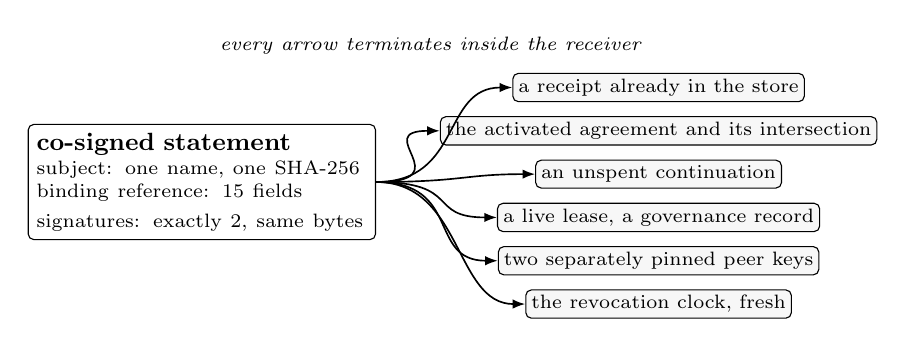
\begin{tikzpicture}[
  font=\small,
  env/.style={draw,rounded corners=2pt,align=center,inner sep=3pt,fill=white},
  rec/.style={draw,rounded corners=2pt,align=left,inner sep=2pt,fill=black!3},
  ptr/.style={-{Latex[length=1.6mm]},semithick},
]
\node[env,align=left,text width=42mm] (stmt) at (0,0)
  {\textbf{co-signed statement}\\[1pt]
   \scriptsize subject: one name, one SHA-256\\
   \scriptsize binding reference: \PSBindingFieldCount{} fields\\
   \scriptsize signatures: exactly 2, same bytes};
\node[rec] (rcpt) at (58mm,12mm) {\scriptsize a receipt already in the store};
\node[rec] (scope) at (58mm,6.5mm) {\scriptsize the activated agreement and its intersection};
\node[rec] (cont)  at (58mm,1mm)  {\scriptsize an unspent continuation};
\node[rec] (lease) at (58mm,-4.5mm) {\scriptsize a live lease, a governance record};
\node[rec] (keys)  at (58mm,-10mm) {\scriptsize two separately pinned peer keys};
\node[rec] (epoch) at (58mm,-15.5mm) {\scriptsize the revocation clock, fresh};
\foreach \t in {rcpt,scope,cont,lease,keys,epoch}{
  \draw[ptr] (stmt.east) .. controls +(11mm,0) and +(-9mm,0) .. (\t.west);
}
\node[font=\scriptsize\itshape,anchor=south] at (29mm,15mm)
  {every arrow terminates inside the receiver};
\end{tikzpicture}
\caption{The mechanism. The statement carries no authority of its own: its
subject, the binding fields the receiver compares, and each of its two keys
resolve only against records the receiving kernel placed in its own stores
before the request arrived.}
\label{fig:mechanism}
\end{figure}


\subsection{Consume, bind, co-sign}

Replay is not defeated by a signature, since a replayed statement is validly
signed. It is defeated by a single-use continuation: a token minted by the
origin binding the parent receipt, the parent session anchor, the capability,
the action class, the target tool, a nonce, the two kernel identities, and a
validity window, whose digest is one of the \PSBindingFieldCount{} bound fields.
The receiver's state machine over it is two operations on one table keyed by the
continuation identifier: \emph{consume} inserts, ignoring a conflict, and reads
the affected row count; zero rows means the continuation was already spent and
the call is denied with \code{chio_treaty_continuation_replay}. \emph{Release}
deletes the row for that identifier and that admission, and runs only when a
later pre-dispatch step denies, so a rejected call does not burn a continuation
the origin will retry. Once dispatch commits the row stays: at-most-once, on
purpose.

The receiver then builds its own admission report and binds the accepted
material into the receipt it is about to sign. One field is treated differently
from the other fourteen: the receiver checks only that
\code{admission_report_sha256} is well-formed hex, then recomputes the digest of its \emph{own} report and overwrites the field before
signing, because a peer-supplied hash must never sit inside a locally signed
receipt as though the receiver had computed it. Verified material is installed
for that one request as a validated value, never as configuration. The local
receipt is persisted; only then does the kernel ask the peer to co-sign a
statement whose subject is the new receipt's digest, so a refusal or a transport
failure is recorded against a receipt that already exists rather than erasing
it.

\section{Security}
\label{sec:security}

Four properties carry the protocol, each over the adversary of
Section~\ref{sec:threat} and reduced to an assumption of
Table~\ref{tab:assumptions}. All four concern the inbound statement; the
outbound one gates the response, never the dispatch.

\paragraph{Admission binding.}
\emph{If a receiving kernel dispatches a federated tool call, then both keys
the activated agreement pins signed the presented statement $S$'s
pre-authentication bytes; every digest the request presented equalled that of
the receiver-stored artifact its identifier resolved to, and $S$'s binding
reference names that digest for the agreement, the intersection, the
continuation and any lineage bundle; every other compared leaf of $S$ equals
what the receiver computed for this request, save two bound to a receiver-held
set, the lease expiry to the instants strictly after the receiver's clock and
the issuer to the agreement's participants; and the continuation $S$ names was
unconsumed at admission.}
Suppose not. Each equality is byte equality between a digest the receiver
computed and one the statement carries, so a difference that passed means two
objects share a SHA-256 image or a canonical encoding, contradicting
ASSUME-SHA256 or the encoder's injectivity under ASSUME-CANONICAL-JSON; a
differing signature contradicts ASSUME-ED25519, a twice-consumed continuation
ASSUME-SQLITE-ATOMICITY. Two residuals remain: completeness follows from
exhaustiveness over the leaf type, and that the shipped hook realizes the
enumerated predicate is a corpus on one fixture, fixing each leaf's kind of
comparison and not the quantity it names.

Nothing in the agreement puts the statement in that antecedent: the resolved
co-signing mode adds the invocation record to required evidence only at exactly
\code{bilateral_required}, nothing at \code{bilateral_if_cross_org}, and never
the statement, which only an explicit required-evidence entry names. The kernel
closes it above the hook, refusing a federated call the hook allowed carrying
no verified statement. One passport key signs three preimages: the receipt
signing body, the co-signing body and the pre-authentication encoding, so
ASSUME-ED25519 carries these properties only with the three disjoint, which
here is structural: a reserved first byte for the encoding, disjoint key sets
for the others.

\paragraph{Receiver locality.}
\emph{Every root, pin, agreement, action-class table and registry used to decide
a request is state the receiver held before the request arrived; the request
selects among them and contributes none.}
Extraction reads a fixed set of key names and ignores the rest; each is an
identifier, the argument of a total lookup over receiver-owned state.

\paragraph{Single use.}
\emph{For a continuation identifier $c$, at most one admission ever reaches
dispatch with $c$ bound to it.}
Under ASSUME-SQLITE-ATOMICITY exactly one of a set of concurrent inserts on a
primary key creates the row; every other denies. Release deletes only the row
keyed by $c$ and the admission that took it, and runs only before dispatch
(Section~\ref{sec:admission}). And $c$ is resident in the receiver's store
before the request, authenticated by residency and digest rather than signature,
so the receiver decides how many authorizations exist. The reference
path mints it there; origin minting, also permitted, owes an
unpredictability premise.

\paragraph{Audience binding.}
\emph{A statement accepted by receiver $R$ is not accepted by a different
receiver $R'$ unless $R'$ activated an identical agreement, resolved the same
intersection, and holds the same continuation unconsumed.}
The receiver's identity enters through the continuation, not the statement's
name for it: the continuation $R'$ resolved names $R'$ as target and both
kernels as participants of the agreement $R'$ activated, which has exactly two,
so $R'$ admits only as its second, under the key it pins. Another
validly co-signed statement from the same pair stops there too, naming a
continuation the receiver does not know or has consumed.

\paragraph{Substitution over the binding reference.}
Table~\ref{tab:subst} is an executed corpus over the \PSBindingFieldCount{}
binding fields, evidence \PSSubstitutionEvidenceId{}; every denial in it leaves
the continuation unconsumed and hands no verified material to dispatch.
\scriptsize
\begin{longtable}{@{}p{3.15cm}p{6.15cm}p{2.75cm}p{1.75cm}@{}}
\caption{Substituting one binding field at a time with a well-formed different value, both signatures valid over the substituted statement, as decided by the pre-dispatch hook. The signer list appears twice, as a set and in order, and the four conditional rows are compared only when the action class's required-evidence set makes the admission resolve the artifact they bind. Each case re-signs with both participant keys, so both signatures verify over the bytes the hook decides on; of the \PSSubstitutionCaseCount{} cases one substitutes nothing and admits, so every denial is attributable to the field that changed. \code{binding_mismatch} and \code{unverified_evidence} abbreviate \code{chio_treaty_dsse_binding_mismatch} and \code{chio_treaty_unverified_required_evidence}.}\label{tab:subst}\\
\toprule
Field & Receiver-side value it must equal & First code & Compared when \\
\midrule
\endfirsthead
\toprule
Field & Receiver-side value it must equal & First code & Compared when \\
\midrule
\endhead
\bottomrule
\endfoot
\code{treaty_id} & the agreement the receiver resolved for this request & \code{binding_mismatch} & always \\
\code{treaty_scope_sha256} & the digest the receiver computes over its own agreement record & \code{binding_mismatch} & always \\
\code{ladder_intersection}\code{_sha256} & the intersection digest the receiver resolved & \code{binding_mismatch} & always \\
\code{admission_report}\code{_sha256} & \emph{nothing}: 64 hex characters, then overwritten by the receiver's own report digest & none: the substituted call is admitted and dispatches & never \\
\code{continuation_sha256} & the resolved continuation's digest & \code{binding_mismatch} & always \\
\code{action_class_id} & the action class the receiver resolved for this request & \code{binding_mismatch} & always \\
\code{consistency_model} & the model the resolved intersection fixed & \code{binding_mismatch} & always \\
\code{request_sha256} & this dispatch's argument hash, and the predicate's own \code{tool_args_hash} & \code{binding_mismatch} & always \\
\code{lease_refs} & the lease in the receiver's own admission bundle & \code{binding_mismatch} & always \\
\code{governance_refs} & the governance record in that bundle & \code{binding_mismatch} & always \\
\code{signer_kernel_ids}, as a set & exactly two, equal as a set to the agreement's participants & \code{binding_mismatch} & always \\
\code{signer_kernel_ids}, in order & the invocation record's order; a reversal resolves the two pinned keys transposed, and strict envelope verification refuses that pairing before the ordered comparison runs & \code{unverified}\code{_evidence} & always \\
\code{lineage_bundle_sha256} & the lineage bundle the receiver resolved & \code{binding_mismatch} & lineage required \\
\code{outcome_sha256} & the outcome digest in the receiver's invocation record & \code{binding_mismatch} & record required \\
\code{local_receipt_sha256} & the lineage bundle's root receipt digest, and the invocation record's & \code{binding_mismatch} & either required \\
\code{remote_receipt_sha256} & the lineage bundle's leaf receipt digest, and the invocation record's & \code{binding_mismatch} & either required \\
\end{longtable}
\normalsize

\noindent
That table is one sub-object of the comparison set, not the set. A strict
statement's wire type has \PSLeafCount{} leaves; the profile refuses
\PSLeafRefusedCount{}, leaving \PSLeafPossibleCount{} a statement may carry and
\PSLeafCarriedCount{} this call carries: \PSLeafEqualityCount{} compared for
equality against a named receiver-held value, \PSLeafDomainCount{} for
membership in a receiver-held set, \PSLeafStatementOnlyCount{} against the
statement alone, by a declared constant or a second leaf, and
\PSLeafUncomparedCount{} against nothing the receiver holds.
\PSPredicateCaseCount{} executed cases fix that classification leaf by leaf.

Those \PSLeafUncomparedCount{} include the report digest, the consistency
anchor, the policy and governance identifiers, and the subject digest, which
only the conforming verifier of Section~\ref{sec:cross} checks. Each is still
held to its declared shape: a substitution within it moves no decision, while a
non-hexadecimal report digest and an empty policy identifier are denied. It is
additive too: the \PSLeafOptionalCount{} optional leaves this call omits are
never read, so an adversary holding both keys adds them and the receiver
admits.

A statement's presentation window is the intersection of three intervals the
receiver itself resolved: the agreement's, the ladder intersection's, and the
continuation's, each revocable and re-scoped per counterparty between calls,
and after the first dispatch it is zero. The lease bounds it only from below,
by the clock comparison above: the hook resolves no lease record and no
governance record, so nothing the receiver stored bounds it above; the lease
registry is the conforming verifier's.

\paragraph{Revocation.}
Revocation is the only part of this protocol that depends on arrival. A kernel
installs an origin's signed snapshot only if its epoch strictly exceeds the
installed one, by compare-and-swap, so neither a replay nor a lost concurrent
install is possible, then applies its own freshness window to the issue time.
Safety holds in every partition because both halves are local predicates that
never wait for a message: no call is allowed against an observed revocation,
and one evaluated against a stale snapshot is denied.

Liveness holds only under ASSUME-GOSSIP-FAIRNESS-PARTITION-BOUND, and bounds the
time before a revocation is observed, not the number of evaluations, which is
unbounded. With $F$ the freshness window, $T$ the control-poll period, $L$
one admitted call's latency, and $k$ the calls made before one is decided
against the newer snapshot, a still-connected receiver denies within $T + kL$ of
publication and a cut receiver within $F + T + kL$, its snapshot first ageing
past $F$. At $F = \PSFreshnessMs$\,ms, $T = \PSEpochTickMs$\,ms and the median
$L$ and $k$ of Section~\ref{sec:eval}, those are
\fpeval{round(\PSEpochTickMs + \PSFedRevokeCallsMedian * \PSFedAllowPFiftyMs, 1)}\,ms
connected and
\fpeval{round(\PSFreshnessMs + \PSEpochTickMs + \PSFedCutCallsMedian * \PSFedAllowPFiftyMs, 1)}\,ms
cut.

\section{What is mechanized}

The decision core is a pure function with no input or output of its own: verify
a capability, resolve the matching grants, evaluate, sign. It is modeled in
Lean 4 \cite{lean4}, and the published theorem inventory carries
\PSTheoremCount{} declarations and one explicit axiom, a symbolic
collision-resistance idealization registered against ASSUME-SHA256. No
serializer, protocol step, or kernel behavior is axiomatized; an unproved
property is an assumption-registry entry, not a hole in the development.

Three results bear on this paper, all bounded. A finite-domain refinement
checker is sound and exact: it succeeds exactly when every receipt in the
supplied finite domain admitted under the amended agreement was admitted under
the prior one. Occurrence theorems make the predicate language fail closed: an
atom that is unsupported, or undefined for the admission view, anywhere in a
predicate forces denial on every view, by induction over the predicate. An
accept-set decomposition shows envelope acceptance is exactly issuer-key trust,
kernel-key trust, and satisfaction of the fail-closed predicate, with signature
validity abstracted into trust-store membership.

\dfn{Lean does not verify the running Rust.} That is the boundary. What exists
instead is four kinds of tripwire, each failing loudly when implementation and
model drift apart: named Rust functions mirrored to named Lean definitions by
content hash and checked on every change; \PSAeneasFunctionCount{} production
functions extracted through a Rust-to-Lean pipeline with equivalence theorems
that must rebuild byte-identically; \PSKaniHarnessCount{} bounded
model-checking harnesses over public entry points, among them ones asserting
that an untrusted issuer is rejected before dispatch and that the signer refuses
a content-digest mismatch; and the cross-language encoder corpus of
Section~\ref{sec:eval}. Distributed revocation has a bounded
model over lossy, duplicating, reordering channels with skew and partition.

We report mutation survivors rather than percentages. Of \PSLeanMutants{}
mutants introduced into the Lean development \PSLeanMutantsKilled{} were killed
and \PSLeanMutantsSurvived{} survived, each with an open issue; of
\PSProofMutants{} introduced into the Rust proof-facing sources
\PSProofMutantsKilled{} were killed, \PSProofMutantsUnviable{} were unviable,
and \PSProofMutantsSurvived{} survived. A survivor is a place where some theorem
is weaker than it looks.

\section{Evaluation}
\label{sec:eval}

Everything below ran on one machine: \PSHostCores{} \PSHostCpuModel{} cores,
\PSHostMemoryGiB{} GiB, \PSHostOs{}, compiler \PSRustcVersion{} at the pinned
toolchain. Percentiles interpolate between order statistics.

\paragraph{Two kernels in separate processes.}
Two kernels were brought up as separate operating-system processes, each
generating its own keys and owning its own stores, issuers, agreements, leases,
and receipt log, with a third process driving calls over \PSFedTransport{}; the
topology record reports \PSFedHosts{} host. The co-signing
and revocation hops are the shipped lanes unchanged; the request hop uses a
transport defined for this experiment, since no shipped lane carries a tool
call. Admitted calls: \PSFedAllowSampleCount{} calls, p50
\PSFedAllowPFiftyMs{} ms, p99 \PSFedAllowPNinetyNineMs{} ms at the driver, each
costing \PSFedCosignConnections{} co-signing connections, counted by the
receiver. Of
that round trip the receiver's evaluation window is
\PSFedReceiverEvalPFiftyMs{} ms at the median and the driver's evidence
preparation \PSFedEvidencePrepPFiftyMs{} ms.

Denied calls: \PSFedDenyCases{} scenarios driven over the wire,
\PSFedDenySampleCount{} calls, p50 \PSFedDenyPFiftyMs{} ms, p99
\PSFedDenyPNinetyNineMs{} ms. They return \code{chio_treaty_missing_scope},
\code{chio_treaty_scope_hash_mismatch},
\code{chio_treaty_missing_intersection},
\code{chio_treaty_intersection_mismatch},
\code{chio_treaty_missing_required_evidence},
\code{request_smuggled_trust_root}, and
\code{request_smuggled_dynamic_trust}. In every one the receiver's dispatch
counter was zero: not one of these calls reached a tool. The latencies are
reported because a denial slower than an allow is an availability problem.

Across the run \PSFedAbsorbedCount{} further calls were denied because the
receiver's snapshot had aged past its \PSFreshnessMs{} ms freshness window while
the origin publishes every \PSEpochTickMs{} ms: \PSFedAllowAbsorbedCount{} of
the \PSFedAllowAttemptCount{} attempts behind the admitted measurement, about
\fpeval{round(100*\PSFedAllowAbsorbedCount/\PSFedAllowAttemptCount,0)} percent,
\PSFedDenyAbsorbedCount{} in the denial experiment, and
\PSFedRevokeAbsorbedCount{} in the revocation experiment. They are the
safety rule of Section~\ref{sec:security} firing on the clock rather than on a
revocation; they were retried and are excluded from the latency distributions.

Revoking at the origin and measuring to the receiver's first denial took
\PSFedRevokeToDenyMs{} ms at the median over \PSFedRevokeRepeats{} repeats, from
\PSFedRevokeMinMs{} to \PSFedRevokeMaxMs{} ms, a median of
\PSFedRevokeCallsMedian{} calls. With the link cut the receiver serves until its
snapshot leaves the freshness window and then denies, \PSFedCutToDenyMs{} ms at
the median over \PSFedCutRepeats{} repeats, from \PSFedCutMinMs{} to
\PSFedCutMaxMs{} ms, a median of \PSFedCutCallsMedian{} calls, counting a
denial only once it persists for three further calls. Both medians sit under the
$k = 1$ bounds of Section~\ref{sec:security}, and every observation, both maxima
included, sits under those bounds evaluated at the largest call count the run
recorded and the admitted p99 latency,
\fpeval{round(\PSEpochTickMs + \PSFedRevokeCallsMax*\PSFedAllowPNinetyNineMs, 1)}\,ms
and
\fpeval{round(\PSFreshnessMs + \PSEpochTickMs + \PSFedCutCallsMax*\PSFedAllowPNinetyNineMs, 1)}\,ms.
The partitioned receiver stops rather than falling back to its last good
answer. On
\PSFedRevokeAmbiguousReleases{} of the \PSFedRevokeDenialRecords{} retained
revoke records and \PSFedCutAmbiguousReleases{} of the
\PSFedCutDenialRecords{} cut records the denial's pre-dispatch release could
not be confirmed and was recorded as ambiguous rather than released, the path
Section~\ref{sec:admission} names; the denial was unaffected and no call
dispatched.

\paragraph{What admission costs locally.}
\begin{table}[!tb]
\centering
\small
\caption{Local cost decomposition. The first two rows are complete kernel paths measured per invocation with both kernels in one process; the rest are components.}
\label{tab:local}
\begin{tabular}{@{}lrrr@{}}
\toprule
Path or component & p50 & p99 or max & samples \\
\midrule
Admitted call, both kernels in one process & \PSPredispatchAllowPFiftyMs{} ms & \PSPredispatchAllowPNinetyNineMs{} ms & \PSPredispatchAllowSampleCount{} \\
Refused before dispatch & \PSPredispatchDenyPFiftyMs{} ms & \PSPredispatchDenyPNinetyNineMs{} ms & \PSPredispatchDenySampleCount{} \\
Receipt append to the store & \PSReceiptAppendPFiftyUs{} us & \PSReceiptAppendPNinetyNineUs{} us & \PSReceiptAppendSampleCount{} \\
Receipt signing & \PSReceiptSignPFiftyUs{} us & \PSReceiptSignMaxUs{} us & \PSReceiptSignSampleCount{} \\
Receipt verification & \PSReceiptVerifyPFiftyUs{} us & \PSReceiptVerifyMaxUs{} us & \PSReceiptVerifySampleCount{} \\
Two-signature statement verification & \PSBilateralVerifyPFiftyUs{} us & \PSBilateralVerifyMaxUs{} us & \PSBilateralVerifySampleCount{} \\
Cross-boundary admission decision & \PSCrossBoundaryPFiftyUs{} us & \PSCrossBoundaryMaxUs{} us & \PSCrossBoundarySampleCount{} \\
\bottomrule
\end{tabular}
\end{table}

The shape of Table~\ref{tab:local} is the finding: the cryptography is not the
expense. Appending the receipt durably costs
\fpeval{round(\PSReceiptAppendPFiftyUs/\PSBilateralVerifyPFiftyUs,1)} times what
verifying the two-signature statement costs, its schema and self-consistency
rules included, and
\fpeval{round(\PSReceiptAppendPFiftyUs/\PSCrossBoundaryPFiftyUs,0)} times the
receiver's decision over already resolved evidence, where the comparisons of
Table~\ref{tab:subst} run. Durability dominates, which is the price of
Section~\ref{sec:admission}'s ordering. The same admission across two processes
costs \PSFedAllowPFiftyMs{} ms; the difference is the transport and the
\PSFedCosignConnections{} co-signing connections, not the decision. One caveat belongs with the refusal
row: its fixture refuses on a unanimous deny verdict, an early exit that never
reaches the comparisons of Table~\ref{tab:subst} or the signature checks, so it
is a lower bound on a refusal. Held at saturation for \PSSustainedSeconds{} s
the same path admitted \PSSustainedCalls{} calls at
\PSSustainedCallsPerSecond{} calls per second with \PSSustainedDenials{}
denials and
\fpeval{round(\PSSustainedReceiptStoreGrowthKiB/1024,1)}\,MiB of receipt-store
growth.

The negative corpus is \PSThreatCaseCount{} in-process cases, each asserting its
expected code; \PSThreatDispatchCaseCount{} run through the dispatch-capable
hook with the tool-invocation counter asserted zero, and the remaining
\PSThreatVerifierCaseCount{} exercise the verifier directly. Alongside it run \PSBilateralReplayCases{} bilateral and
\PSGenericReplayCases{} generic replay cases.

\paragraph{Verification by someone who was not there.}
The \PSProofPackageKiB{} KiB evidence package for the refund workflow verifies with
no access to either kernel, every receipt, statement, lease, and governance
record, in \fpeval{round(\PSBuyerVerifyPFiftyUs/1000,1)}\,ms at the median over
\PSBuyerVerifySampleCount{} runs. A frozen corpus of \PSVectorCaseCount{}
receipt cases holds \PSVectorLanguages{} independent implementations, in Rust,
TypeScript, Python, and Go, to the same canonical body bytes and verdict.

\paragraph{Reproduction.}
Every measurement above was taken at commit \code{\PSRunCommit{}}. The
cross-process run's environment
record marks its worktree \PSFedWorktreeState{}; what differed were the retained
result files written by the benchmark that ran before it, and no source file. Each run writes its environment record, raw samples, and the
macro file this paper compiles from, so a printed and a retained number cannot
drift.

\section{Limitations and related work}

The cross-organization run of Section~\ref{sec:eval} put the two kernels in
separate processes on one host, not on two separately administered machines.
That removes the shared address space, store, and key material, which are what
the claim is about; the shared operating system and clock source remain, and
removing them changes the latencies. The rule does not depend on that
experiment; the strength of the demonstration does.

Section~\ref{sec:eval}'s alternative is one construction of those parts on one
corpus, and its request schema is ours, so what it measures is what an operator
must add, not a bound on what the parts reach.
Continuation consumption is at-most-once, so a crash between consume and
dispatch loses the call rather than repeating it: right for a refund, an
avoidable retry for an idempotent read. The chain closes in the kernel for one
hop: the next continuation in a longer chain is minted outside it.
Denial paths below the verifier still return a rendered detail alongside the
code; separating them is unfinished. Receipts batch into
Merkle checkpoints in the RFC 6962 shape \cite{rfc6962} with offline inclusion
proofs, and that is the whole claim: local audit evidence with verifiable
inclusion, not a public append-only log, with no anti-equivocation, so a
kernel signing two contradictory checkpoints is detectable only
by someone holding both.

\paragraph{Related work.}
Capability discipline without ambient authority is the tradition this protocol
sits in \cite{saltzer1975,watson2010capsicum}, saying exactly where a proof
stops is seL4's discipline \cite{sel4}, and attenuable credentials are old and
good: trust management \cite{spki,keynote}, macaroons
\cite{macaroons}, and the modern token families \cite{ucan,biscuit}, which carry
caveats without a kernel, a decision record, or a price. Kerberos
\cite{kerberos} crosses the boundary by transferring authority, workload
identity by minting a local credential for a foreign workload \cite{spiffe},
and token exchange by converting one issuer's token into another's
\cite{rfc8693}: all three move authority, which is the step this protocol
declines to take. Interchain light
clients \cite{ibc} solve pinned keys plus a monotone clock for chains, not tool
calls, and policy engines decide from a request they are handed
\cite{cedar}. The envelope shapes we reuse \cite{dsse,intoto},
transparent registration \cite{scitt}, and certificate transparency
\cite{rfc6962} answer how an artifact was built, who may register a statement,
and how to publish verifiable records. None of them defines the object that is
at once the authorization decision, the audit record, the accounting entry, and
the evidence another organization's kernel verifies against state it alone
holds.

\paragraph{What we believe.}
The rule is smaller than the system that implements it, and we think it is the
part that lasts. The receiver decides from facts only it holds; which names must
cross follows from that decision rather than preceding it, and the record has to
outlive the connection and be checkable by someone who trusts neither side.


{\scriptsize\linespread{0.93}\selectfont
\setlength{\bibsep}{0.3pt plus 0.2ex}
\bibliographystyle{plain}
\bibliography{bib}}

\end{document}
